{The strength $S$ of a wooden beam is directly proportional to its cross sectional  width $w$ and the square of its height $h$; that is, $S = kwh^2$ for some constant $k$. 

\noindent\begin{minipage}{\linewidth}
\centering
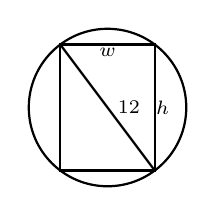
\begin{tikzpicture}
\draw [thick](0,0) circle (1cm);
\draw [thick](-.6,.8) -- node [pos=.5,right] {\scriptsize $12$} (.6,-.8);
\draw [thick](-.6,-.8) rectangle (.6,.8);
\draw (.7,0) node {\scriptsize $h$} (0,.7) node {\scriptsize $w$};
\end{tikzpicture}
\end{minipage}

Given a circular log with diameter of 12 inches, what sized beam can be cut from the log with maximum strength?
}
{$w=4\sqrt{3}$, $h=4\sqrt{6}$
}

